\documentclass[10pt,a4paper]{article}
\usepackage[UTF8,fontset = windows]{ctex}
\setCJKmainfont[BoldFont=黑体,ItalicFont=楷体]{华文中宋}
\usepackage{amssymb,amsmath,amsfonts,amsthm,mathrsfs,dsfont,graphicx}
\usepackage{ifthen,indentfirst,enumerate,color,titletoc}
\usepackage{tikz}
\usetikzlibrary{arrows,calc,intersections,patterns}
\usepackage[bf,small,indentafter,pagestyles]{titlesec}
\usepackage[top=1in, bottom=1in,left=0.8in,right=0.8in]{geometry}
\begin{document}
\begin{center}
\begin{tikzpicture}[>=latex]
    \draw [->] (-1,0) -- (4,0) node [below] {$x$};
    \draw [->] (0,-1) -- (0,3) node [left] {$y$};
    \draw (0,1) arc (90:0:1) -- (3,2);
    \draw (0,0) node [below left] {$O$};
    \draw (1,0) node [below] {$1$};
    \draw (0,1) node [left] {$1$};
    \draw [dashed] (2,0) -- (2,1) -- (0,1);
    \draw (2,0) node [below] {$2$};
\end{tikzpicture}
\end{center}

\begin{center}
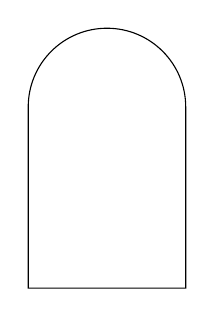
\begin{tikzpicture}[>=latex]
    \draw (0,0) -- (2,0) -- (2,2.3) arc (0:180:1) -- cycle;
\end{tikzpicture}
\end{center}

\begin{center}
\begin{tikzpicture}[>=latex]
    \draw [->] (-1,0) -- (6,0) node [below] {$x$};
    \draw [->] (0,-2.5) -- (0,2.5) node [left] {$y$};
    \draw (2,0) node [below] {$2$};
    \draw (5,0) node [above] {$5$};
    \draw [domain = 0:2,samples = 100] plot (\x,-\x*\x+2*\x);
    \draw [domain = 2:5,samples = 100] plot (\x, \x*\x/2-4*\x+6);
    \draw [dashed] (5,0) -- (5,-1.5);
    \draw (0,0) node [below left] {$O$};
\end{tikzpicture}
\end{center}

\begin{center}
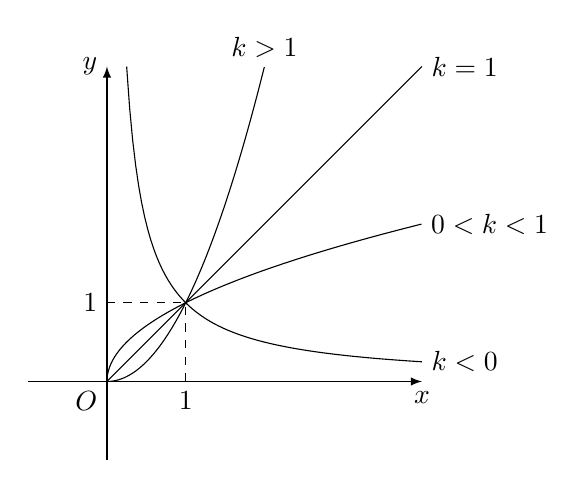
\begin{tikzpicture}[>=latex]
    \draw [->] (-1,0) -- (4,0) node [below] {$x$};
    \draw [->] (0,-1) -- (0,4) node [left] {$y$};
    \draw (0,0) node [below left] {$O$};
    \draw (0,0) -- (4,4) node [right] {$k=1$};
    \draw [domain = 0.25:4, samples = 100] plot (\x, 1/\x) node [right] {$k<0$};
    \draw [domain = 0:2, samples = 100] plot (\x,\x*\x) node [above] {$k>1$};
    \draw [domain = 0:2, samples = 100] plot (\x*\x,\x) node [right] {$0<k<1$};
    \draw [dashed] (1,0) node [below] {$1$} -- (1,1) -- (0,1) node [left] {$1$};
\end{tikzpicture}
\end{center}

\begin{center}
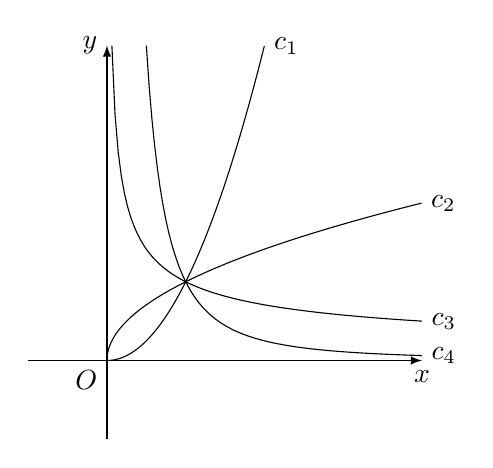
\begin{tikzpicture}[>=latex]
    \draw [->] (-1,0) -- (4,0) node [below] {$x$};
    \draw [->] (0,-1) -- (0,4) node [left] {$y$};
    \draw (0,0) node [below left] {$O$};
    \draw [domain = 0:2, samples = 100] plot (\x,\x*\x) node [right] {$c_1$};
    \draw [domain = 0:2, samples = 100] plot (\x*\x,\x) node [right] {$c_2$};
    \draw [domain = 0.0625:4, samples = 100] plot (\x, {1/sqrt(\x)}) node [right] {$c_3$};
    \draw [domain = 0.5:4, samples = 100] plot (\x, {1/\x/\x}) node [right] {$c_4$};
\end{tikzpicture}
\end{center}

\begin{center}
\begin{tikzpicture}[>=latex]
    \draw [->] (-3,0) -- (3,0) node [below] {$x$};
    \draw [->] (0,-3) -- (0,3) node [left] {$y$};
    \draw (0,0) node [below right] {$O$};
    \draw [domain = {-3^(1/4)}:{3^(1/4)}] plot (\x*\x*\x,\x*\x*\x*\x);
    \draw (0,-3) node [below] {(A)};
\end{tikzpicture}
\end{center}

\begin{center}
\begin{tikzpicture}[>=latex]
    \draw [->] (-3,0) -- (3,0) node [below] {$x$};
    \draw [->] (0,-3) -- (0,3) node [left] {$y$};
    \draw (0,0) node [below right] {$O$};
    \draw [domain = {-3^(1/5)}:{3^(1/5)}] plot (\x*\x*\x,\x*\x*\x*\x*\x);
    \draw (0,-3) node [below] {(B)};
\end{tikzpicture}
\end{center}

\begin{center}
\begin{tikzpicture}[>=latex]
    \draw [->] (-3,0) -- (3,0) node [below] {$x$};
    \draw [->] (0,-3) -- (0,3) node [left] {$y$};
    \draw (0,0) node [below right] {$O$};
    \draw [domain = {0}:{3^(1/3)}] plot (\x*\x,\x*\x*\x);
    \draw (0,-3) node [below] {(C)};
\end{tikzpicture}
\end{center}

\begin{center}
\begin{tikzpicture}[>=latex]
    \draw [->] (-3,0) -- (3,0) node [below] {$x$};
    \draw [->] (0,-3) -- (0,3) node [left] {$y$};
    \draw (0,0) node [below right] {$O$};
    \draw [domain = {3^(-3/2)}:3] plot (\x,{\x^(-2/3)}) plot (-\x,{\x^(-2/3)});
    \draw (0,-3) node [below] {(D)};
\end{tikzpicture}
\end{center}

\begin{center}
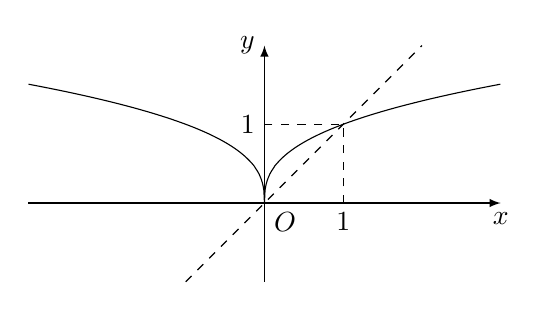
\begin{tikzpicture}[>=latex]
    \draw [->] (-3,0) -- (3,0) node [below] {$x$};
    \draw [->] (0,-1) -- (0,2) node [left] {$y$};
    \draw (0,0) node [below right] {$O$};
    \draw [dashed] (-1,-1) -- (2,2);
    \draw [domain = 0:3, samples = 400] plot (\x,{\x^(3/8)}) plot (-\x,{\x^(3/8)});
    \draw [dashed] (1,0) node [below] {$1$} -- (1,1) -- (0,1) node [left] {$1$};
\end{tikzpicture}
\end{center}

\begin{center}
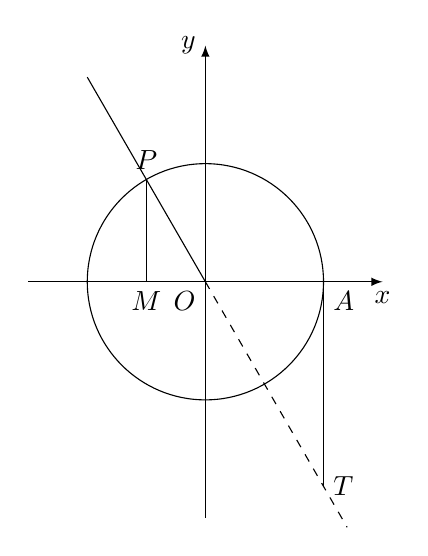
\begin{tikzpicture}[>=latex,scale = 1.5]
    \draw [->] (-1.5,0) -- (1.5,0) node [below] {$x$};
    \draw [->] (0,-2) -- (0,2) node [left] {$y$};
    \draw (0,0) node [below left] {$O$} circle (1);
    \draw (1,0) node [below right] {$A$} -- (1,{-sqrt(3)}) node [right] {$T$};
    \draw (-0.5,0) node [below] {$M$} -- (-0.5,{sqrt(3)/2}) node [above] {$P$};
    \draw (-1,{sqrt(3)}) -- (0,0);
    \draw [dashed] (0,0) -- (1.2,{-1.2*sqrt(3)});
\end{tikzpicture}
\end{center}

\begin{center}
\begin{tikzpicture}[>=latex, scale = 1.8]
    \draw [->] (-1.5,0) -- (1.5,0) node [below] {$x$};
    \draw [->] (0,-1.5) -- (0,1.5) node [left] {$y$};
    \draw (0,0) node [below left] {$O$};
    \draw (0,0) circle (1);
\end{tikzpicture}
\end{center}

\begin{center}
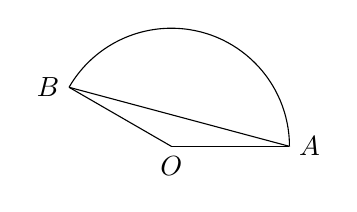
\begin{tikzpicture}[>=latex,scale = 1.5]
    \draw (0,0) node [below] {$O$} -- (1,0) node [right] {$A$};
    \draw (1,0) -- (150:1) node [left] {$B$};
    \draw (150:1) -- (0,0);
    \draw (1,0) arc (0:150:1);
\end{tikzpicture}
\end{center}

\begin{center}
\begin{tikzpicture}[>=latex]
    \draw (0,0) coordinate (O) node [below] {$O$};
    \draw ({90-51.79}:3) coordinate (C) node [right] {$C$};
    \draw ({90+51.79}:3) coordinate (A) node [left] {$A$};
    \draw ({90+51.79}:{48/49}) coordinate (D) node [left] {$D$};
    \draw (A) -- (O) -- (C) arc ({90-51.79}:{90+51.79}:3) (C) -- (D);
\end{tikzpicture}
\end{center}

\begin{center}
\begin{tikzpicture}[>=latex]
    \draw (0,0) node [below left] {$D$} -- (4,0) node [below] {$C$} -- (7,0) node [below right] {$B$} -- (7,3) node [above right] {$A$};
    \draw (4,0) -- (7,3);
    \draw (0,0) -- (7,3);
    \draw (4.5,0) arc (0:atan(1):0.5);
    \draw (5,0) node [above] {$\alpha$};
    \draw (0.5,0) arc(0:atan(3/7):0.5);
    \draw (1.5,0) node [above] {$\beta$};
\end{tikzpicture}
\end{center}

\begin{center}
\begin{tikzpicture}[>=latex, line cap = round, scale = 0.5]
    \draw (0,0) -- (0,5.5) node [left] {$A$} coordinate (A);
    \draw (0,5.5) -- ++ (45:{4*sqrt(2)}) coordinate (B) node [right] {$B$};
    \draw (A) ++ ({45-asin(1/sqrt(26))}:{sqrt(13)}) coordinate (C) node [right] {$C$} -- (B);
    \draw (C) -- (A);
\end{tikzpicture}
\end{center}

\begin{center}
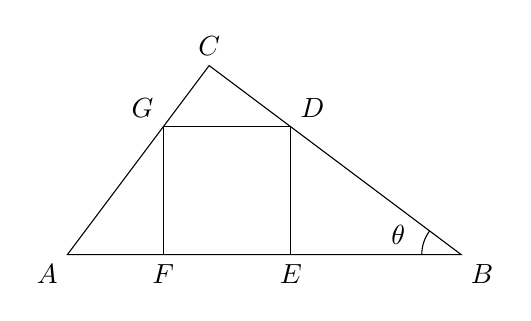
\begin{tikzpicture}[>=latex, line cap = round]
    \draw (0,0) node [below left] {$A$}-- (5,0) node [below right] {$B$}-- (9/5,12/5) node [above] {$C$}-- cycle;
    \draw (45/37,0) node [below] {$F$} -- (45/37,60/37) node [above left] {$G$}-- (105/37,60/37) node [above right] {$D$}-- (105/37,0) node [below] {$E$}; 
    \draw (5,0) ++ (180:0.5) arc (180:180-atan(3/4):0.5); 
    \draw (4.2,0) node [above] {$\theta$};
\end{tikzpicture}
\end{center}

\begin{center}
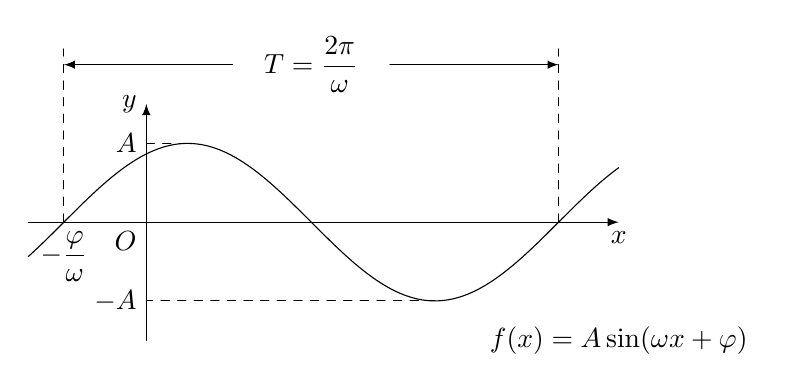
\begin{tikzpicture}[>=latex, line cap = round]
    \draw [->] (-1.5,0) -- (6,0) node [below] {$x$};
    \draw [->] (0,-1.5) -- (0,1.5) node [left] {$y$};
    \draw (0,0) node [below left] {$O$};
    \draw [domain = -1.5:6, samples = 1000] plot (\x,{sin(\x/pi*180+60)});
    \draw [dashed] (pi/6,1) -- (0,1)  node [left] {$A$} (pi/6+pi,-1) -- (0,-1) node [left] {$-A$};
    \draw (6,-1.5) node {$f(x)=A\sin (\omega x+\varphi)$};
    \draw [dashed] (-pi/3,0) -- (-pi/3,2.2) (5*pi/3,0) -- (5*pi/3,2.2);
    \draw [->] (2*pi/3-1,2) -- (-pi/3,2);
    \draw [->] (2*pi/3+1,2) -- (5*pi/3,2);
    \draw (2*pi/3,2) node {$T=\dfrac{2\pi}{\omega}$};
    \draw (-pi/3,0) node [below] {$-\dfrac{\varphi}{\omega}$};
\end{tikzpicture}
\end{center}

\begin{center}
\begin{tikzpicture}[>=latex, line cap = round, scale = 0.8]
    \draw [->] (-1,0) -- (7,0) node [below] {$x$};
    \draw [->] (0,-3) -- (0,3) node [left] {$y$};
    \draw (0,0) node [below right] {$O$};
    \draw [domain = -pi/6:25*pi/12, samples = 1000] plot (\x, {2*sin(2*\x/3/pi*180+20)});
    \draw [dashed] (7*pi/12,2) -- (0,2) node [left] {$2$};
    \draw [dashed] (25*pi/12,0) node [above] {$\dfrac{25\pi}{12}$} --++ (0,-2) -- (0,-2) node [left] {$-2$};
    \draw (-pi/6,0) node [below] {$-\dfrac{\pi}{6}$};
\end{tikzpicture}
\end{center}

\begin{center}
\begin{tikzpicture}[>=latex, line cap = round, scale = 0.4]
    \draw [->] (-4,0) -- (11,0) node [below] {$x$};
    \draw [->] (0,-5) -- (0,5) node [left] {$y$};
    \draw (0,0) node [below right] {$O$};
    \draw [domain = -2:11, samples = 1000] plot (\x, {-4*sin(180*\x/8+45)});
    \draw [dashed] (2,-4) -- (0,-4) node [left] {$-4$} (10,4) -- (0,4) node [left] {$4$};
    \draw (-2,0) node [above] {$-2$};
    \draw (6,0) node [below] {$6$};
\end{tikzpicture}
\end{center}

\begin{center}
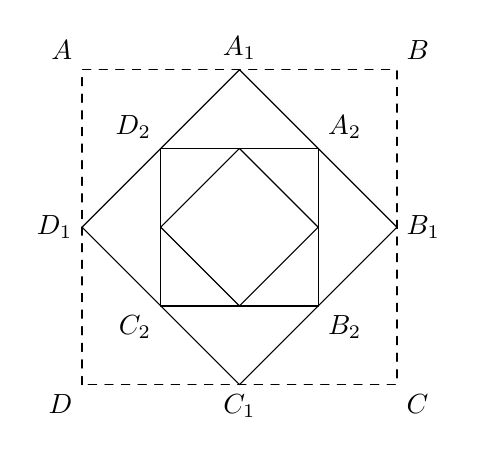
\begin{tikzpicture}[>=latex, line cap = round, line join = round]
    \draw [dashed] (0,0) rectangle (4,4);
    \draw (0,2) -- (2,4) -- (4,2) -- (2,0) -- cycle;
    \draw (1,3) -- (3,3) -- (3,1) -- (1,1) -- cycle;
    \draw (2,3) -- (3,2) -- (2,1) -- (1,2) -- cycle;
    \draw (0,4) node [above left] {$A$} (4,4) node [above right] {$B$} (4,0) node [below right] {$C$} (0,0) node [below left] {$D$};
    \draw (2,4) node [above] {$A_1$} (4,2) node [right] {$B_1$} (2,0) node [below] {$C_1$} (0,2) node [left] {$D_1$};
    \draw (3,3) node [above right] {$A_2$} (3,1) node [below right] {$B_2$} (1,1) node [below left] {$C_2$} (1,3) node [above left] {$D_2$};
\end{tikzpicture}
\end{center}

\begin{center}
\begin{tikzpicture}[>=latex, line cap = round, line join = round, scale = 1.5]
    \draw (0,0) node [below left] {$A$} -- (2,0) node [below right] {$B$}-- (3,1) node [above right] {$C$} -- (1,1) node [above left] {$D$}-- cycle;
\end{tikzpicture}
\end{center}

\begin{center}
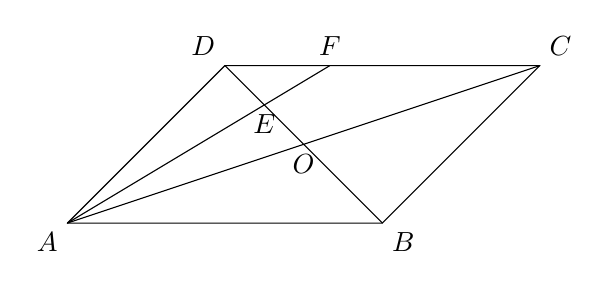
\begin{tikzpicture}[>=latex, line cap = round, line join = round, scale = 2]
    \draw (0,0) node [below left] {$A$} -- (2,0) node [below right] {$B$}-- (3,1) node [above right] {$C$} -- (1,1) node [above left] {$D$}-- cycle;
    \draw (0,0) -- (3,1) (2,0) -- (1,1);
    \draw (0,0) -- (5/3,1) node [above] {$F$};
    \draw (1.5,0.5) node [below] {$O$};
    \draw (1.25,0.75) node [below] {$E$};
\end{tikzpicture}
\end{center}

\begin{center}
\begin{tikzpicture}[>=latex, line cap = round, line join = round, scale = 1.5]
    \draw (0,0) -- (3,0) (0,1) node [above left] {$A$} -- (4,1) (1,-1) -- (2,-1) (2,2) node [above left] {$C$} -- (4,2);
    \draw (0,0) -- (0,1) (1,-1) -- (1,1) (2,-1) -- (2,2) (3,0) -- (3,2) (4,1) -- (4,2);
    \draw (0,1) -- (1,0) node [below right] {$B$} coordinate (B) (2,2) -- (3,1) node [below right] {$D$};
    \draw [dashed] (B) --++ (45:1/2) --++ (1,0) --++ (225:1/2);
    \draw [dashed] (B) ++ (0,1) --++ (45:1/2) --++ (1,0) --++ (225:1/2);
    \draw [dashed] (B) ++ (45:1/2) --++ (0,1) ++ (1,0) --++ (0,-1);
\end{tikzpicture}
\end{center}

\begin{center}
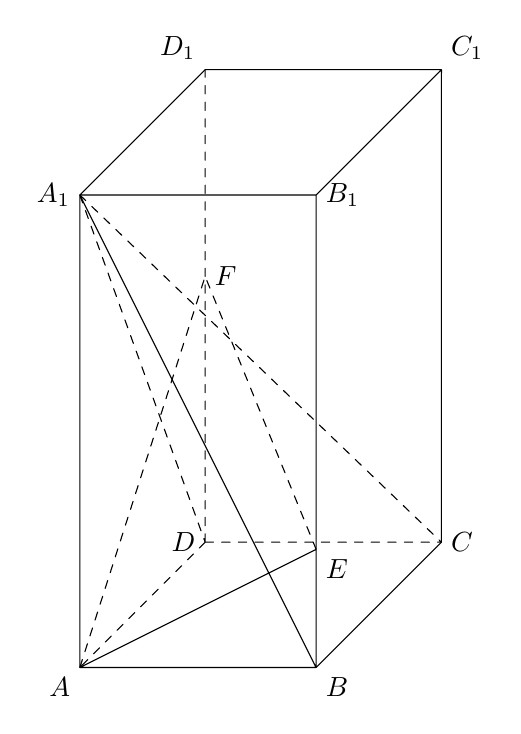
\begin{tikzpicture}[>=latex, line cap = round, line join = round, scale = 1.5]
    \draw (0,0) coordinate (A) node [below left] {$A$};
    \draw (A) ++ (2,0) coordinate (B) node [below right] {$B$};
    \draw (A) ++ (45:1.5) coordinate (D) node [left] {$D$};
    \draw (D) ++ (2,0) coordinate (C) node [right] {$C$};
    \draw (B) ++ (0,1) coordinate (E) node [below right] {$E$};
    \draw (D) ++ (0,9/4) coordinate (F) node [right] {$F$};
    \draw (A) ++ (0,4) coordinate (A1) node [left] {$A_1$};
    \draw (B) ++ (0,4) coordinate (B1) node [right] {$B_1$};
    \draw (C) ++ (0,4) coordinate (C1) node [above right] {$C_1$};
    \draw (D) ++ (0,4) coordinate (D1) node [above left] {$D_1$};
    \draw (A) -- (B) -- (C) -- (C1) -- (D1) -- (A1) -- cycle (C1) -- (B1) -- (B) (B1) -- (A1) (A1) -- (B) (A) -- (E);
    \draw [dashed] (D) -- (A) (D) -- (C) (D) -- (D1) (A1) -- (C) (A) -- (F) -- (E) (A1) -- (D);
\end{tikzpicture}
\end{center}

\begin{center}
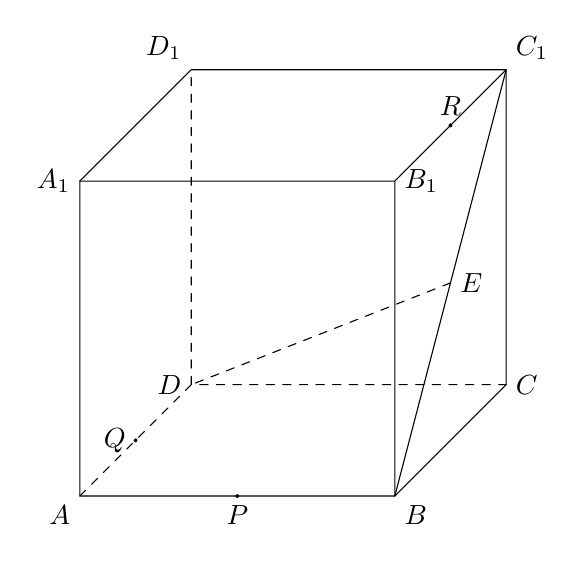
\begin{tikzpicture}[>=latex, line cap = round, line join = round]
    \draw (0,0) node [below left] {$A$} coordinate (A) -- (4,0) node [below right] {$B$} coordinate (B) --++ (45:{4/2}) node [right] {$C$} coordinate (C)
    --++ (0,4) node [above right] {$C_1$} coordinate (C1)
    --++ (-4,0) node [above left] {$D_1$} coordinate (D1) --++ (225:{4/2}) node [left] {$A_1$} coordinate (A1) -- cycle;
    \draw (4,4) node [right] {$B_1$} coordinate (B1) -- (B) (B1) --++ (45:{4/2}) (B1) --++ (-4,0);
    \draw [dashed] (0,0) --++ (45:{4/2}) node [left] {$D$} coordinate (D) --++ (4,0) (D) --++ (0,4);
    \draw (C1) -- (B);
    \draw ($(B)!0.5!0:(C1)$) node [right] {$E$} coordinate (E);
    \draw [dashed] (E) -- (D);
    \filldraw ($(A)!0.5!0:(B)$) node [below] {$P$} circle (0.02);
    \filldraw ($(A)!0.5!0:(D)$) node [left] {$Q$} circle (0.02);
    \filldraw ($(B1)!0.5!0:(C1)$) node [above] {$R$} circle (0.02);
\end{tikzpicture}
\end{center}

\begin{center}
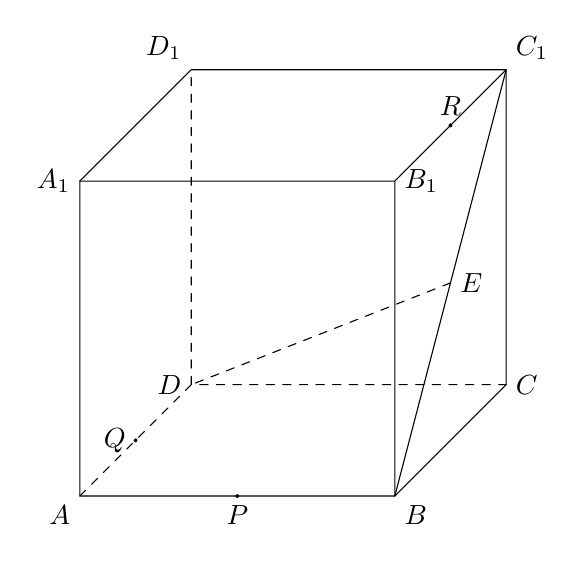
\begin{tikzpicture}[>=latex, line cap = round, line join = round]
    \draw (0,0) node [below left] {$A$} coordinate (A) -- (4,0) node [below right] {$B$} coordinate (B) --++ (45:{4/2}) node [right] {$C$} coordinate (C)
    --++ (0,4) node [above right] {$C_1$} coordinate (C1)
    --++ (-4,0) node [above left] {$D_1$} coordinate (D1) --++ (225:{4/2}) node [left] {$A_1$} coordinate (A1) -- cycle;
    \draw (4,4) node [right] {$B_1$} coordinate (B1) -- (B) (B1) --++ (45:{4/2}) (B1) --++ (-4,0);
    \draw [dashed] (0,0) --++ (45:{4/2}) node [left] {$D$} coordinate (D) --++ (4,0) (D) --++ (0,4);
    \draw (C1) -- (B);
    \draw ($(B)!0.5!0:(C1)$) node [right] {$E$} coordinate (E);
    \draw [dashed] (E) -- (D);
    \filldraw ($(A)!0.5!0:(B)$) node [below] {$P$} circle (0.02);
    \filldraw ($(A)!0.5!0:(D)$) node [left] {$Q$} circle (0.02);
    \filldraw ($(B1)!0.5!0:(C1)$) node [above] {$R$} circle (0.02);
\end{tikzpicture}
\end{center}

\begin{center}
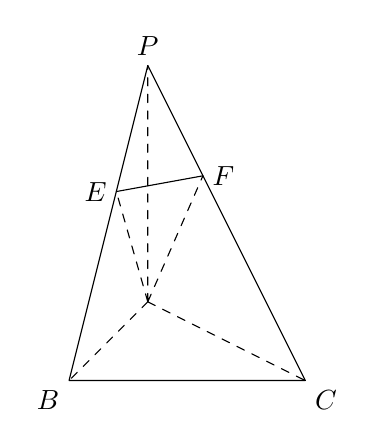
\begin{tikzpicture}[>=latex, line cap = round, line join = round]
    \draw (0,0) coordinate (B) (3,0) coordinate (C) (1,1) coordinate (A) (1,4) coordinate (P);
    \draw (B) node [below left] {$B$} -- (C) node [below right] {$C$} -- (P) node [above] {$P$} -- cycle;
    \draw ($(B)!0.6!0:(P)$) coordinate (E) node [left] {$E$} ($(C)!0.65!0:(P)$) coordinate (F) node [right] {$F$};
    \draw (E) -- (F);
    \draw [dashed] (A) -- (P) (A) -- (B) (A) -- (C) (A) -- (E) (A) -- (F); 
\end{tikzpicture}
\end{center}

\begin{center}
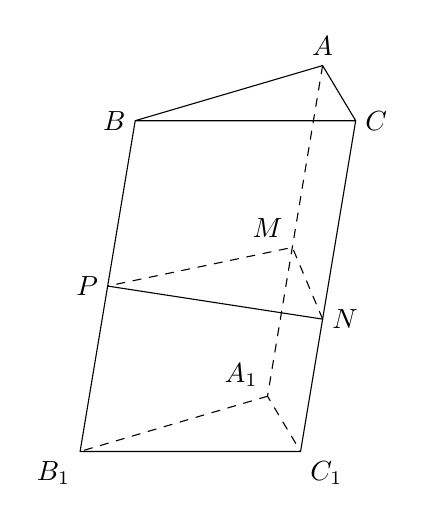
\begin{tikzpicture}[>=latex, line cap = round, line join = round, scale = 1.4]
    \draw (0,0) node [below left] {$B_1$} coordinate (B1) -- (2,0) node [below right] {$C_1$} coordinate (C1) 
    -- ++ (0.5,3) node [right] {$C$} coordinate (C) --++ (-2,0) node [left] {$B$} coordinate (B) -- cycle;
    \draw (B) --++ (1.7,0.5) node [above] {$A$} coordinate (A) -- (C);
    \draw [dashed] (A) --++ (-0.5,-3) node [above left] {$A_1$} coordinate (A1) -- (C1) (A1) -- (B1);
    \draw ($(B)!0.5!0:(B1)$) node [left] {$P$} coordinate (P);
    \draw ($(C)!0.6!0:(C1)$) node [right] {$N$} coordinate (N);
    \draw ($(A)!0.55!0:(A1)$)node [above left] {$M$} coordinate (M);
    \draw (P) -- (N);
    \draw [dashed] (N) -- (M) -- (P);
\end{tikzpicture}
\end{center}

\begin{center}
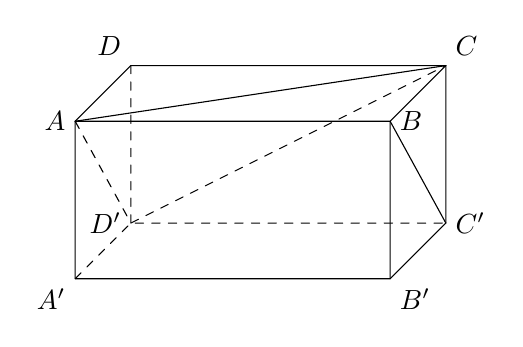
\begin{tikzpicture}[>=latex, line cap = round, line join = round, scale = 2]
    \draw (0,0) node [below left] {$A'$} coordinate (AP) --++ (2,0) node [below right] {$B'$} coordinate (BP) --++ (45:{1/2}) node [right] {$C'$} coordinate (CP)
    --++ (0,1) node [above right] {$C$} coordinate (C)
    --++ (-2,0) node [above left] {$D$} coordinate (D) --++ (225:{1/2}) node [left] {$A$} coordinate (A) -- cycle;
    \draw (AP) ++ (2,1) node [right] {$B$} coordinate (B) -- (BP) (B) --++ (45:{1/2}) (B) --++ (-2,0);
    \draw [dashed] (AP) --++ (45:{1/2}) node [left] {$D'$} coordinate (DP) --++ (2,0) (DP) --++ (0,1);
    \draw (B) -- (CP) (A) -- (C);
    \draw [dashed] (A) -- (DP) -- (C);
\end{tikzpicture}
\end{center}

\begin{center}
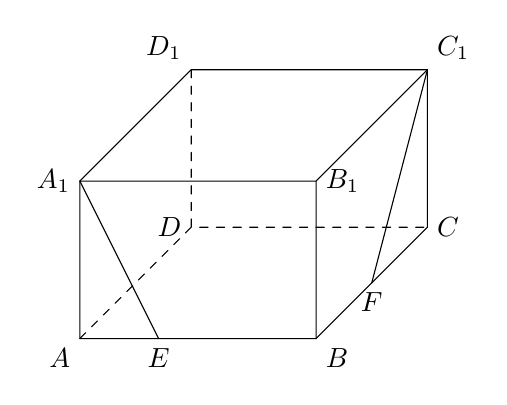
\begin{tikzpicture}[>=latex, line cap = round, line join = round, scale = 1]
    \draw (0,0) node [below left] {$A$} coordinate (A) --++ (3,0) node [below right] {$B$} coordinate (B) --++ (45:{4/2}) node [right] {$C$} coordinate (C)
    --++ (0,2) node [above right] {$C_1$} coordinate (C1)
    --++ (-3,0) node [above left] {$D_1$} coordinate (D1) --++ (225:{4/2}) node [left] {$A_1$} coordinate (A1) -- cycle;
    \draw (A) ++ (3,2) node [right] {$B_1$} coordinate (B1) -- (B) (B1) --++ (45:{4/2}) (B1) --++ (-3,0);
    \draw [dashed] (A) --++ (45:{4/2}) node [left] {$D$} coordinate (D) --++ (3,0) (D) --++ (0,2);
    \draw ($(A)!{1/3}!0:(B)$) node [below] {$E$} -- (A1);
    \draw ($(B)!{1/2}!0:(C)$) node [below] {$F$} -- (C1);
\end{tikzpicture}
\end{center}

\begin{center}
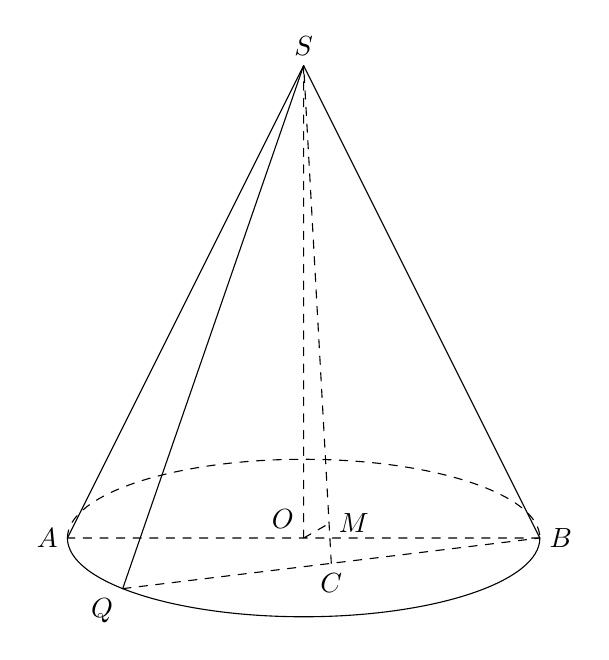
\begin{tikzpicture}[>=latex, line cap = round, line join = round, scale = 1]
    \draw (-3,0) node [left] {$A$} arc (180:360:3 and 1) node [right] {$B$} -- (0,6) coordinate (S) node [above] {$S$} -- cycle;
    \draw [dashed] (-3,0)  arc (180:0:3 and 1);
    \draw ({-3*cos(40)},{-sin(40)}) node [below left] {$Q$} coordinate (Q) -- (0,6);
    \draw [dashed] (Q) -- (3,0) coordinate (B);
    \draw [dashed] ($(Q)!0.5!0:(B)$) node [below] {$C$} coordinate (C) -- (S) -- (0,0) node [above left] {$O$} coordinate (O);
    \draw [dashed] (O) -- ($(C)!0.08!0:(S)$) node [right] {$M$} (B) -- (-3,0);
\end{tikzpicture}
\end{center}

\begin{center}
\begin{tikzpicture}[>=latex, line cap = round, line join = round, scale = 1]
    \draw (0,0) node [below] {$B$} --++ (1,{sqrt(3)}) node [above right] {$C$} --++ (-2,0) node [above left] {$A$} -- cycle;
    \draw [dashed] (-2,0) node [below left] {$P_1$} -- (2,0) node [below right] {$P_2$} -- (0,{2*sqrt(3)}) node [above] {$P_3$} -- cycle;
\end{tikzpicture}
\end{center}

\begin{center}
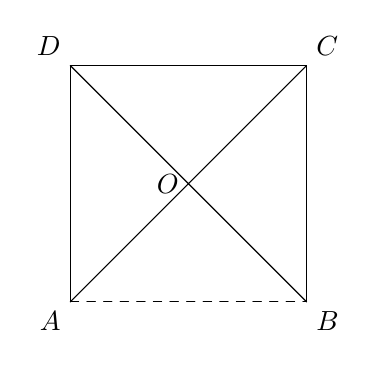
\begin{tikzpicture}[>=latex, line cap = round, line join = round, scale = 1]
    \draw (0,0) node [below left] {$A$} -- (0,3) node [above left] {$D$} -- (3,3) node [above right] {$C$} -- (3,0) node [below right] {$B$};
    \draw (0,0) -- (3,3) (3,0) -- (0,3) (1.5,1.5) node [left] {$O$};
    \draw [dashed] (0,0) -- (3,0);
\end{tikzpicture}
\end{center}

\begin{center}
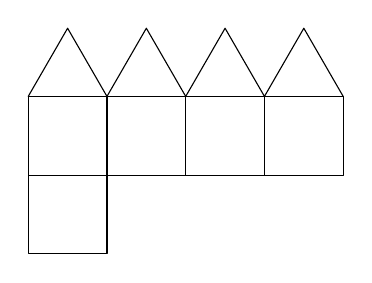
\begin{tikzpicture}[>=latex, line cap = round, line join = round, scale = 1]
    \draw (0,0) -- (4,0) -- (4,1) -- (0,1) -- cycle;
    \draw (0,0) -- (0,-1) -- (1,-1) -- (1,1) (2,1) -- (2,0) (3,1) -- (3,0);
    \draw (0,1) --++ ({1/2},{1/2*sqrt(3)}) --++ ({1/2},{-1/2*sqrt(3)}) --++ ({1/2},{1/2*sqrt(3)}) --++ ({1/2},{-1/2*sqrt(3)}) --++ ({1/2},{1/2*sqrt(3)}) --++ ({1/2},{-1/2*sqrt(3)})
    --++ ({1/2},{1/2*sqrt(3)}) --++ ({1/2},{-1/2*sqrt(3)});
\end{tikzpicture}
\end{center}

\begin{center}
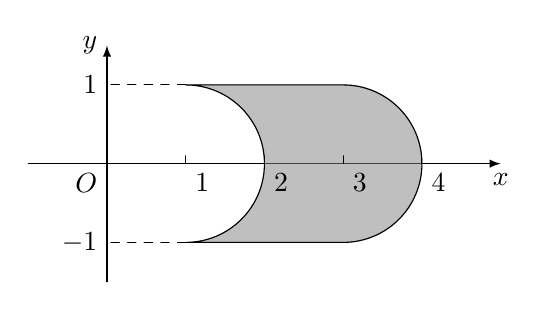
\begin{tikzpicture}[>=latex, line cap = round, line join = round, scale = 1]
    \draw [->] (-1,0) -- (5,0) node [below] {$x$};
    \draw [->] (0,-1.5) -- (0,1.5) node [left] {$y$};
    \draw (0,0) node [below left] {$O$};
    \foreach \i in {-1,1}
    {\draw (0,\i) node [left] {$\i$};}
    
    \filldraw [opacity = 0.5, color = gray] (1,-1) -- (3,-1) arc (270:450:1) -- (1,1) arc (450:270:1); 
    \draw (1,-1) -- (3,-1) arc (270:450:1) -- (1,1) arc (450:270:1); 
    \foreach \i in {1,2,...,4}
    {\draw (\i,0.1) -- (\i,0) node [below right] {$\i$};}
    \draw [dashed] (1,1) -- (0,1) (1,-1) -- (0,-1);
\end{tikzpicture}
\end{center}

\begin{center}
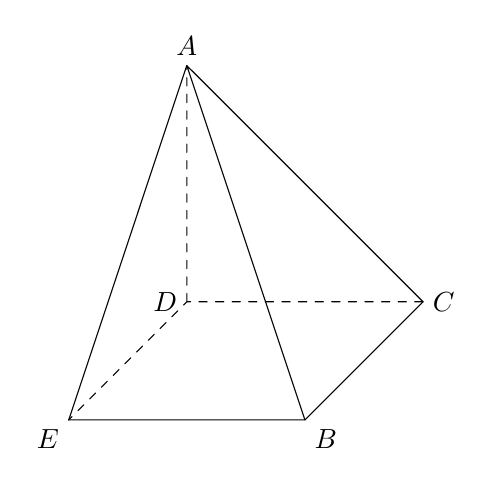
\begin{tikzpicture}[>=latex, line cap = round, line join = round, scale = 3]
    \draw (0,0) node [below left] {$E$} -- (1,0) node [below right] {$B$} --++ (45:{sqrt(2)/2}) node [right] {$C$} coordinate (C);
    \draw [dashed] (C) --++ (-1,0) node [left] {$D$} coordinate (D) -- (0,0) (D) --++ (0,1) node [above] {$A$} coordinate (A);
    \draw (A) -- (0,0) (A) -- (C) (A) -- (1,0);
\end{tikzpicture}
\end{center}

\begin{center}
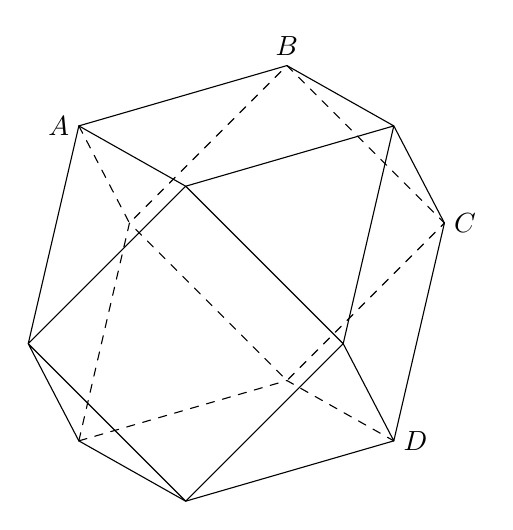
\begin{tikzpicture}[>=latex, line cap = round, line join = round]
    \draw (0,0) coordinate(M) (4,0) coordinate (N) (N) ++ (50:2) coordinate (P) (M) ++ (50:2) coordinate (Q);
    \draw (M) ++ (0,4) coordinate (M1) (N) ++ (0,4) coordinate (N1) (P) ++ (0,4) coordinate (P1) (Q) ++ (0,4) coordinate (Q1);
    \draw ($(N)!0.5!0:(P)$) coordinate (D) node [right] {$D$} -- ($(M)!0.5!0:(N)$) coordinate (D1) -- ($(M)!0.5!0:(Q)$) coordinate (D2);
    \draw [dashed] (D2) -- ($(P)!0.5!0:(Q)$) coordinate (D3) -- (D);
    \draw ($(P)!0.5!0:(P1)$) coordinate (C) node [right] {$C$} -- (D) -- ($(N)!0.5!0:(N1)$) coordinate (C1) -- (D1) -- ($(M)!0.5!0:(M1)$) coordinate (C2) -- (D2);
    \draw [dashed] (D2) -- ($(Q1)!0.5!0:(Q)$) coordinate (C3) -- (D3) -- (C);
    \draw ($(N1)!0.5!0:(P1)$) coordinate (A1) -- ($(P1)!0.5!0:(Q1)$) coordinate (B) node [above] {$B$} -- ($(M1)!0.5!0:(Q1)$) coordinate (A) node [left] {$A$} 
    -- ($(M1)!0.5!0:(N1)$) coordinate (B1) --  cycle;
    \draw (C) -- (A1) -- (C1) -- (B1) -- (C2) -- (A);
    \draw [dashed] (A) -- (C3) -- (B) -- (C);
    
\end{tikzpicture}
\end{center}

\begin{center}
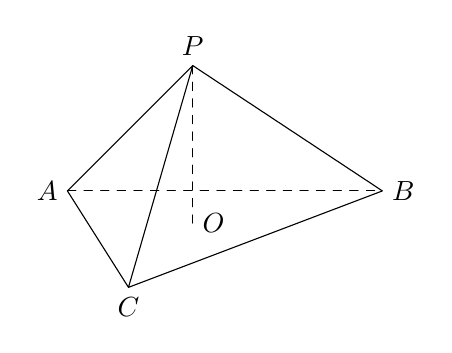
\begin{tikzpicture}[>=latex, line cap = round, line join = round]
    \draw (0,0) coordinate (A) node [left] {$A$} (4,0) coordinate (B) node [right] {$B$};
    \draw (2,0) ++ (225:{sqrt(3)}) coordinate (C) node [below] {$C$};
    \draw (2,0) ++ (225:{sqrt(3)/3}) coordinate (O) node [right] {$O$};
    \draw (O) ++ (0,2) coordinate (P) node [above] {$P$};
    \draw (A) -- (C) -- (B) -- (P) -- (A) (P) -- (C);
    \draw [dashed] (A) -- (B) (P) -- (O);
    
\end{tikzpicture}
\end{center}

\begin{center}
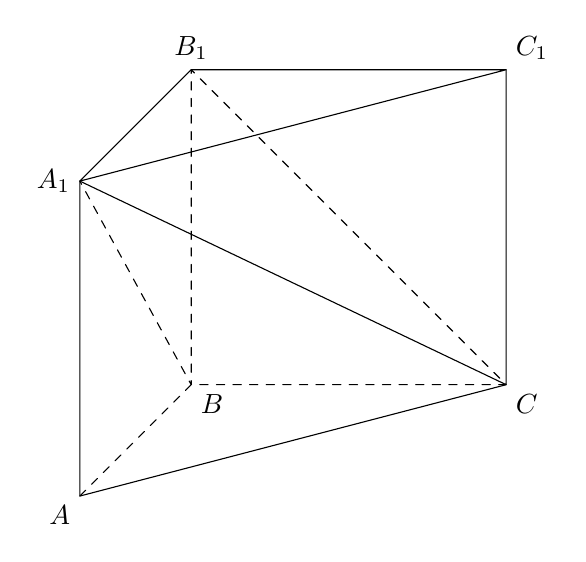
\begin{tikzpicture}[>=latex, line cap = round, line join = round]
    \draw (0,0) node [below left] {$A$} coordinate (A) ++ (45:2) node [below right] {$B$} coordinate (B) 
    ++ (4,0) node [below right] {$C$} coordinate (C);
    \draw (A) ++ (0,4) coordinate (A1) node [left] {$A_1$};
    \draw (B) ++ (0,4) coordinate (B1) node [above] {$B_1$};
    \draw (C) ++ (0,4) coordinate (C1) node [above right] {$C_1$};
    \draw (A1) -- (B1) -- (C1) -- cycle;
    \draw (C1) -- (C) -- (A) -- (A1) -- (C);
    \draw [dashed] (A) -- (B) -- (C) -- (B1)-- (B) -- (A1);
    
\end{tikzpicture}
\end{center}

\begin{center}
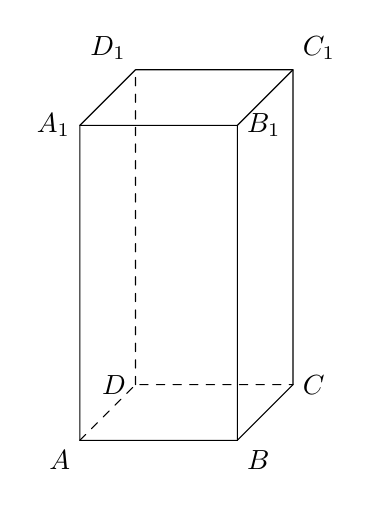
\begin{tikzpicture}[>=latex, line cap = round, line join = round, scale = 2]
    \draw (0,0) node [below left] {$A$} coordinate (A) --++ (1,0) node [below right] {$B$} coordinate (B) --++ (45:{1/2}) node [right] {$C$} coordinate (C)
    --++ (0,2) node [above right] {$C_1$} coordinate (C1)
    --++ (-1,0) node [above left] {$D_1$} coordinate (D1) --++ (225:{1/2}) node [left] {$A_1$} coordinate (A1) -- cycle;
    \draw (A) ++ (1,2) node [right] {$B_1$} coordinate (B1) -- (B) (B1) --++ (45:{1/2}) (B1) --++ (-1,0);
    \draw [dashed] (A) --++ (45:{1/2}) node [left] {$D$} coordinate (D) --++ (1,0) (D) --++ (0,2);
    
    
\end{tikzpicture}
\end{center}

\begin{center}
\begin{tikzpicture}[>=latex, line cap = round, line join = round, scale = 2]
    \draw ({-sqrt(3)},0) coordinate (A) node [left] {$A$};
    \draw ({sqrt(3)},0) coordinate (C) node [right] {$C$};
    \draw (45:0.5) coordinate (D) node [above right] {$D$};
    \draw (225:0.5) coordinate (B) node [below left] {$B$};
    \draw (0,{sqrt(3)}) coordinate (P) node [above] {$P$};
    \draw ($(P)!0.5!0:(B)$) coordinate (E) node [left] {$E$};
    \draw (A) -- (B) -- (C) -- (P) -- (A) (P) -- (B);
    \draw [dashed] (D) -- (A) (D) -- (E) (D) -- (C) (D) -- (P);
\end{tikzpicture}
\end{center}

\begin{center}
\begin{tikzpicture}[>=latex, line cap = round, line join = round, scale = 1.2]
    \draw [->] (-2,0) -- (6.5,0) node [below] {成绩(分)};
    \draw [->] (0,-1) -- (0,3) node [left] {$\dfrac{\text{频率}}{\text{组距}}$};
    \draw (0,0) node [below left] {$O$};
    \draw (1,0) -- (1,0.5) -- (2,0.5);
    \draw (2,0) -- (2,1) -- (3,1);
    \draw (3,0) -- (3,2) -- (4,2) -- (4,0);
    \draw (4,1.5) -- (5,1.5) -- (5,0);
    \draw [dashed] (0,0.5) -- (1,0.5) (0,1) -- (2,1) (0,1.5) -- (4,1.5) (0,2) -- (3,2);
    \foreach \i in {20,40,...,100}
        \draw ({\i/20},0) node [below] {$\i$};
    \foreach \i in {0.005,0.01,0.015,0.02}
        \draw (-1.2,{\i*100}) node [right] {$\i$};
    
\end{tikzpicture}
\end{center}

\begin{center}
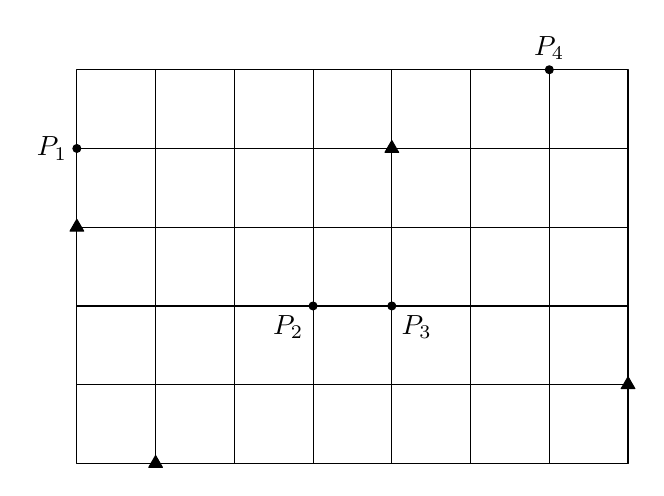
\begin{tikzpicture}[>=latex, line cap = round, line join = round]
    \foreach \i in {0,1,...,7}
        \draw (\i,0) -- (\i,5);
    \foreach \i in {0,1,...,5}
        \draw (0,\i) -- (7,\i);
    \filldraw (0,4) circle (0.05) node [left] {$P_1$};
    \filldraw (3,2) circle (0.05) node [below left] {$P_2$};
    \filldraw (4,2) circle (0.05) node [below right] {$P_3$};
    \filldraw (6,5) circle (0.05) node [above] {$P_4$};
    \filldraw (1,0) ++ (210:0.1) --++ ({0.1*sqrt(3)},0) --++ (120:{0.1*sqrt(3)}) -- cycle;
    \filldraw (0,3) ++ (210:0.1) --++ ({0.1*sqrt(3)},0) --++ (120:{0.1*sqrt(3)}) -- cycle;
    \filldraw (4,4) ++ (210:0.1) --++ ({0.1*sqrt(3)},0) --++ (120:{0.1*sqrt(3)}) -- cycle;
    \filldraw (7,1) ++ (210:0.1) --++ ({0.1*sqrt(3)},0) --++ (120:{0.1*sqrt(3)}) -- cycle;
\end{tikzpicture}
\end{center}

\begin{center}
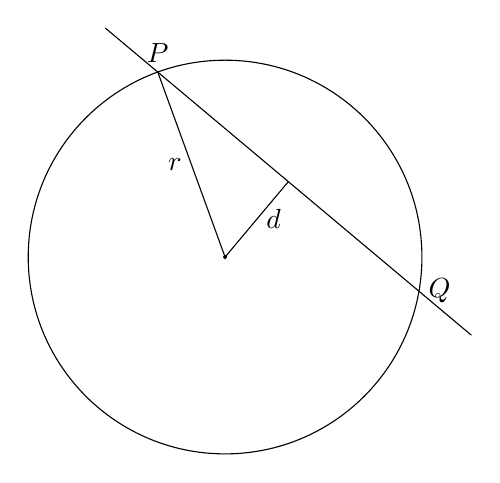
\begin{tikzpicture}[>=latex, line cap = round, line join = round]
    \draw (0,0) circle (2.5);
    \draw (110:2.5) node [above] {$P$} coordinate (P);
    \draw (-10:2.5) node [right] {$Q$} coordinate (Q);
    \filldraw (0,0) circle (0.02);
    \draw ($(P)!0.5!0:(Q)$) -- (0,0) -- (P);
    \draw ($($(P)!0.5!0:(Q)$)!0.5!0:(0,0)$) node [right] {$d$};
    \draw ($(P)!0.5!0:(0,0)$) node [left] {$r$};
    \draw ($(P)!-0.2!0:(Q)$) -- ($(P)!1.2!0:(Q)$);
\end{tikzpicture}
\end{center}

\begin{center}
\begin{tikzpicture}[>=latex, line cap = round, line join = round, scale = 1.5]
    \draw [->] (-0.5,0) -- (4,0) node [below] {$x$};
    \draw [->] (0,-2) -- (0,2) node [left] {$y$};
    \draw (0,0) node [below left] {$O$};    
    \draw [domain = -1.8:1.8, samples = 1000] plot (\x*\x, \x);
    \draw (1.44,1.2) node [above] {$M$};
    \draw (0.49,-0.7) node [below] {$E$} -- (1.44,1.2) -- (2.89,-1.7) node [below] {$F$} -- cycle;
    \draw (0.84,0) node [below right] {$A$} (2.04,0) node [above right] {$B$};
\end{tikzpicture}
\end{center}

\begin{center}
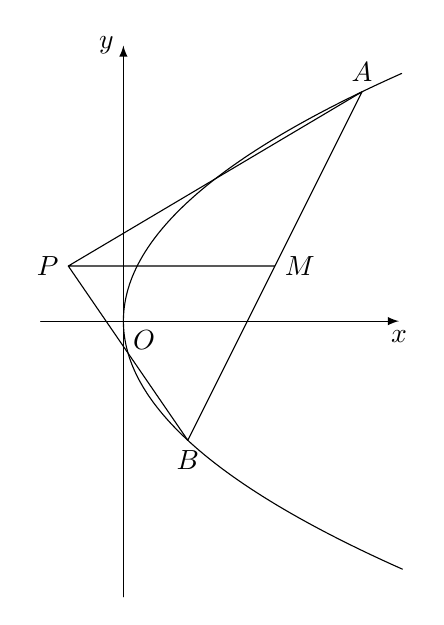
\begin{tikzpicture}[>=latex, line cap = round, line join = round, scale = 0.7]
    \draw [->] (-1.5,0) -- (5,0) node [below] {$x$};
    \draw [->] (0,-5) -- (0,5) node [left] {$y$};
    \draw (0,0) node [below right] {$O$};    
    \draw [domain = -4.5:4.5, samples = 1000] plot (\x*\x/4, \x);
    \draw ({11/4+sqrt(10)/2},{1+sqrt(10)}) node [above] {$A$} coordinate (A);
    \draw ({11/4-sqrt(10)/2},{1-sqrt(10)}) node [below] {$B$} coordinate (B);
    \draw ($(A)!0.5!0:(B)$) node [right] {$M$} coordinate (M);
    \draw (-1,1) node [left] {$P$} coordinate (P);
    \draw (P) -- (M) (A) -- (P) -- (B) -- cycle;

\end{tikzpicture}
\end{center}
\end{document}